%%%%%%%%%%%%%%%%%%%%%%%%%%%%%%%%%%%%%%%%%%%%%%%%%%%%%%%%%%%%%%%%%%%%%%%%%%%%%%%%
% Version Control Systems
%
% Author: FOSSEE 
% Copyright (c) 2009, FOSSEE, IIT Bombay
%%%%%%%%%%%%%%%%%%%%%%%%%%%%%%%%%%%%%%%%%%%%%%%%%%%%%%%%%%%%%%%%%%%%%%%%%%%%%%%%

\documentclass[14pt,compress]{beamer}

\mode<presentation>
{
  \usetheme{Warsaw}
  \useoutertheme{infolines}
  \setbeamercovered{transparent}
}

\usepackage[english]{babel}
\usepackage[latin1]{inputenc}
%\usepackage{times}
\usepackage[T1]{fontenc}

% Taken from Fernando's slides.
\usepackage{ae,aecompl}
\usepackage{mathpazo,courier,euler}
\usepackage[scaled=.95]{helvet}

\definecolor{darkgreen}{rgb}{0,0.5,0}

\usepackage{listings}
\lstset{language=bash,
    basicstyle=\ttfamily\bfseries,
    commentstyle=\color{red}\itshape,
  stringstyle=\color{darkgreen},
  showstringspaces=false,
  keywordstyle=\color{blue}\bfseries}

%%%%%%%%%%%%%%%%%%%%%%%%%%%%%%%%%%%%%%%%%%%%%%%%%%%%%%%%%%%%%%%%%%%%%%
% Macros
\setbeamercolor{emphbar}{bg=blue!20, fg=black}
\newcommand{\emphbar}[1]
{\begin{beamercolorbox}[rounded=true]{emphbar} 
      {#1}
 \end{beamercolorbox}
}
\newcounter{time}
\setcounter{time}{0}
\newcommand{\inctime}[1]{\addtocounter{time}{#1}{\tiny \thetime\ m}}

\newcommand{\typ}[1]{\lstinline{#1}}

\newcommand{\kwrd}[1]{ \texttt{\textbf{\color{blue}{#1}}}  }

% Title page
\title[Mercurial]{Version Control with \typ{hg}}

\author[FOSSEE] {FOSSEE}

\institute[IIT Bombay] {Department of Aerospace Engineering\\IIT Bombay}
\date[]{}

\AtBeginSection[]
{
  \begin{frame}<beamer>
    \frametitle{Outline}
    \tableofcontents[currentsection,currentsubsection]
  \end{frame}
}

%%%%%%%%%%%%%%%%%%%%%%%%%%%%%%%%%%%%%%%%%%%%%%%%%%%%%%%%%%%%%%%%%%%%%%
% DOCUMENT STARTS
\begin{document}

\begin{frame}
  \maketitle
\end{frame}

% CREATING TOC 
\begin{frame}
  \frametitle{Outline}
  \tableofcontents
  % You might wish to add the option [pausesections]
\end{frame}

\begin{frame}
  \frametitle{Objectives}
  At the end of this session, you will be able to:
  \begin{itemize}
  \item Understand what is Version Control and the need for it
  \item Create and use repository on a daily basis
  \item Clone existing repositories, from the web
  \item View the history of a repository 
  \item Make changes to a repository and commit them
  \item Work collaboratively with a team 
  \end{itemize}
\end{frame}

%% There are some %$ used just to minimise the effect of $ sign used
%% in lstlisting. In emacs it looks dirty. 

% Introduction to course-need of version control, history, options available.
\section{Introduction}

\begin{frame}
  \frametitle{What is Version Control?}
  \begin{block}{}
    A way to track changes made to files over time, by keeping copies
    of files as we change them.
  \end{block}
\end{frame}

%% Home made version control system?
\begin{frame}[fragile]
  \frametitle{Home-brewed}
  \begin{center}
    An example of a \typ{home-brew} Version Control system
    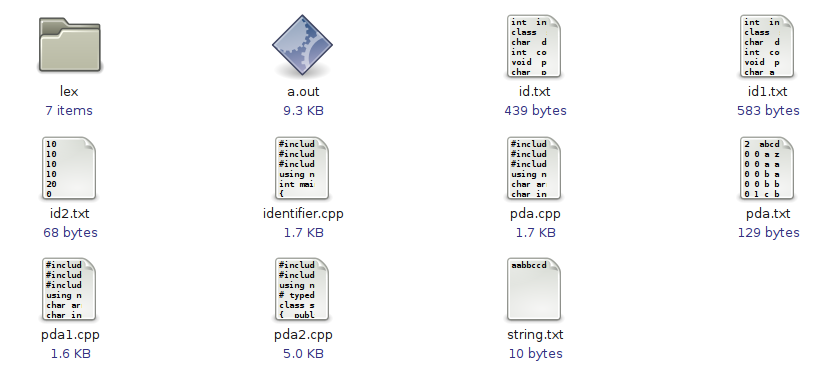
\includegraphics[height=1.8in,width=4.2in]{images/folder.png}
  \end{center}
  \begin{lstlisting} 
$ ls
a.out  id1.txt  id2.txt  identifier.cpp  id.txt  lex  pda1.cpp  pda2.cpp  pda.cpp  pda.txt  string.txt
  \end{lstlisting} %%$
    %%a screen-shot of folder with all crazy names.
\end{frame}

\begin{frame}[fragile]
  \frametitle{Problems}  
  \begin{block}{}    
  \begin{itemize}
  \item Name and changes made are not related or linked. 
  \item Can't track sequence of changes made to a file. 
  \item Does not scale. 
  \end{itemize}
    \end{block}
\end{frame}

\begin{frame}[fragile]
  \frametitle{The need for Version Control}
  \begin{itemize}
  \item \alert{To err is Human} \ldots 
  \item Tracking the history and evolution of a project
  \item To collaborate effectively on a project
  \item To efficiently track down bugs and pin-point the changes that
    caused it 
  \end{itemize}
\end{frame}

%% Introduction to how logs are managed in VCS.
%% A analogy in logs and day-to-day life?
\begin{frame}[fragile]
  \frametitle{How does it work? --- Analogy}
  It is, in some ways, similar to playing an Video game.
  \begin{itemize}
  \item We play games in stages
  \item Once we finish a stage or a task -- \alert{we SAVE}
  \item We continue playing
  \item But, if necessary, we could choose from one of the saved
    states and start from there
  \item We could alter the course of the game
  \end{itemize}
\end{frame}


\begin{frame}
  \frametitle{Mercurial or \typ{hg}}
  \begin{center}
    
\includegraphics[height=.75in,interpolate=true]{images/mercurial_logo}
  \end{center}
  \begin{itemize}
  \item Easy to learn and use
  \item Lightweight
  \item Scales excellently
  \item Written in Python
  \end{itemize}
\end{frame}

\begin{frame}
  \frametitle{Installation}
  \begin{itemize}
  \item \typ{sudo apt-get install mercurial}
  \item TortoiseHg
  \item \typ{\$ hg}
  \item \typ{\$ hg version}
  \end{itemize}
\end{frame}

\section{Let there be a Repo!}
% init, status, commit, log, [ui]
\begin{frame}
  \frametitle{We need a repo!}
  \begin{itemize}
  \item A Repository (repo) is where all the action is!
  \item Project files along with a special directory that stores all the
    changes
  \item We take snapshots of the whole repository; not individual
    files. 
  \end{itemize}
\end{frame}

\begin{frame}
  \frametitle{Initializing a repo}
  \begin{itemize}
  \item \typ{\$ hg init}
  \item Creates a fresh repository
  \item Adds a \typ{.hg} directory to our \emph{working directory}
  \end{itemize}
  \emphbar{\typ{.hg} directory keeps log of changes made henceforth}
\end{frame}

\begin{frame}
  \frametitle{Status report}
  \begin{itemize}
  \item \typ{hg status} gives the status of our repo
  \item Use it often; at least as a beginner
  \item \typ{hg help command} gives us help about \typ{command}
  \end{itemize}
\end{frame}

\begin{frame}[fragile]
  \frametitle{Status codes}
  \begin{lstlisting}
    M = modified                                               
    A = added                                                  
    R = removed                                                
    C = clean                                                  
    ! = missing 
    ? = not tracked                                            
    I = ignored                                                
  \end{lstlisting}
\end{frame}

\begin{frame}
  \frametitle{Adding files}
  \begin{itemize}
  \item From \typ{hg status} we know, none of the files are being
    tracked, yet. 
  \item \typ{hg add} --- asking \typ{hg} to track these files
  \item As expected \typ{hg status} prepends an \typ{A} to the file
  names.
  \item \typ{? --> A} 
  \item \typ{! --> R} (\typ{hg remove})
  \end{itemize}
\end{frame}

\begin{frame}
  \frametitle{Taking Snapshots}
  \begin{itemize}
  \item \typ{hg commit}
  \item Asking Mercurial to take a snapshot; remember the changes made
    to the repository. 
  \item \typ{-u FirstName LastName <email>}
  \item \typ{-m ``Commit message''} -- a description of changes committed. 
  \end{itemize}
\end{frame}

\begin{frame}
  \frametitle{Thumbnail views}
  \begin{itemize}
  \item \typ{hg log}~ gives the log of the changes made
  \item A \typ{changeset} is an atomic collection of changes to the
    files (between successive commits)
  \end{itemize}
  \begin{block}{Log information}
    \begin{itemize}
    \item \alert{changeset}: Identifier for the changeset
    \item \alert{user}: Details of user who created the changeset
    \item \alert{date}: Date and time of creation
    \item \alert{summary}: One line description
    \end{itemize}    
  \end{block}
\end{frame}

\begin{frame}
  \frametitle{User information}
  \begin{itemize}
  \item User information is set in the \typ{hgrc} file
  \item It can be set globally or local to the project
  \item Global \typ{hgrc}
    \begin{itemize}
    \item \typ{\$HOME/.hgrc} -- Unix like systems
    \item \typ{\%HOME\%\\.hgrc} -- Windows
    \end{itemize}
  \end{itemize}
\end{frame}

\begin{frame}
  \frametitle{\alert{Advice}: \typ{commits}, messages}
  \begin{itemize}
  \item Atomic changes; one change with one \typ{commit}
  \item Single line summary --- 60 to 65 characters long
  \item Followed by paragraphs of detailed description
    \begin{itemize}
    \item Why the change?
    \item What does it effect?
    \item Known bugs/issues?
    \item etc. 
    \end{itemize}
  \end{itemize}
\end{frame}

\section{But Why \typ{commit}~?}

\begin{frame}
  \frametitle{Operational overhead?}
  \begin{itemize}
  \item But why do we \typ{commit}?
  \item Isn't all this just adding to operational costs?
  \item Isn't all this a waste of time?
  \end{itemize}
  \begin{center}
    \emphbar{No! You shall see the benefits, soon!}    
  \end{center}
\end{frame}

\begin{frame}
  \frametitle{Revert Changes}
  \begin{itemize}
  \item Undo all changes; the editor can only do so much.
  \item \typ{hg revert --all}
  \item \typ{hg revert filename}
  \item Present file, with changes --- \typ{filename.orig}
  \end{itemize}
\end{frame}

\begin{frame}[fragile]
  \frametitle{Viewing Changes}
  \begin{itemize}
  \item \typ{hg diff} --- all changes since last commit
  \end{itemize}
  \begin{block}{}
    \begin{lstlisting}
      - this line was deleted
      + this line was added
    \end{lstlisting}
  \end{block}
\end{frame}


\begin{frame}[fragile]
  \frametitle{Revision numbering}
  \begin{itemize}
  \item \typ{changeset:   n:cbf6e2a375b4}
  \item \typ{n} is the revision number
  \item The revision number is local to a repository
  \item \typ{cbf6e2a375b4} is the unique identifier
  \end{itemize}
\end{frame}

\begin{frame}[fragile]
  \frametitle{Using revision numbers}
  \begin{itemize}
  \item \typ{-r n} can be passed as arguments to commands to specify
    the revision number
  \item For instance, \typ{hg diff -r1 -r2}
  \item \typ{m:n} specifies a range of revision numbers
  \item For instance, \typ{hg log -r0:2}
  \end{itemize}
\end{frame}

\section{Collaborating with Mercurial}
\begin{frame}[fragile]
  \frametitle{Cloning Repositories}
  \begin{itemize}
  \item \typ{hg clone SOURCE [DEST]}
  \item All \typ{hg} repositories are self-contained
  \end{itemize}
\end{frame}

\begin{frame}[fragile]
  \frametitle{Sharing Repositories}
  \begin{itemize}
  \item \typ{hg serve}
  \item Can be cloned with \typ{hg clone http://my-ip-address:8000}
  \item We share a central repository; work on our local copies. 
  \item Set write permissions in \typ{.hg/hgrc}
  \end{itemize}
  \begin{lstlisting}
    [web]
    push_ssl=False
    allow_push=*
  \end{lstlisting}
\end{frame}

\begin{frame}
  \frametitle{Sharing Changes}
  \begin{itemize}
  \item Use \typ{hg push} to push your \typ{commits}
    (\typ{changesets}) to the central repository
  \end{itemize}
\end{frame}


\begin{frame}
  \frametitle{Pulling Changes}
  \begin{itemize}
  \item \typ{hg incoming} shows new \typ{changesets} in the server 
  \item To get these \typ{changesets}, we use \typ{hg pull}
  \item These changes do not affect our working directory
  \item \typ{hg parent} shows the parents of the working directory
  \end{itemize}
\end{frame}

\begin{frame}
  \frametitle{Pulling Changes \ldots}
  \begin{itemize}
  \item \typ{hg update} will update the working directory 
    \begin{itemize}
    \item Updates to the \typ{tip} if no revision is specified
    \item \typ{tip} is the most recently added changeset 
    \item Can specify revision number to update to
    \end{itemize}
  \item \typ{hg tip} shows the \typ{tip} of the repository
  \end{itemize}
\end{frame}

\begin{frame}
  \frametitle{Simultaneous Changes}
  \begin{itemize}
  \item The logs of both repositories will be different
  \item The repositories have diverged
  \item \typ{hg push} fails, in such a scenario
  \item \alert{Never, Never, Never, Ever} use \typ{hg push -f}
  \end{itemize}
\end{frame}

\begin{frame}
  \frametitle{Merging}
  \begin{itemize}
  \item Pull and merge, when \typ{abort: push creates new remote
    heads!}
  \item \typ{hg merge} will merge the two diverged heads
  \item \typ{commit} after you have \typ{merged}!
  \end{itemize}
\end{frame}

\begin{frame}
  \frametitle{Simultaneous Changes \ldots}
  \begin{itemize}
  \item \typ{outgoing} shows the \typ{changesets} that will be pushed
  \item \typ{hg push} works!
  \item Look at the `Change graph'!
  \end{itemize}
\end{frame}

\begin{frame}
  \frametitle{Simultaneous Conflicting Changes}
  \begin{itemize}
  \item What if the changes conflict? -- overlapping edits
  \item \typ{hg push} fails; \typ{hg pull}; \typ{hg merge}
  \item You now get a diff view with 3 panes 
    \begin{itemize}
    \item First --- current file
    \item Second --- \typ{changesets} that you pulled
    \item Third --- file before you made your changes
    \end{itemize}
  \item Resolve conflict and save
  \item \typ{hg commit}; \typ{hg push}
  \item Look at the `Change graph'!
  \end{itemize}
\end{frame}

\section{Conclusion}

\begin{frame}
  \frametitle{\alert{Advice}: Work-flow}
  General work-flow
  \begin{itemize}
  \item \typ{pull}; \typ{update}
  \item Make changes
  \item \typ{commit}
  \item If changes on repo, \typ{pull} and \typ{merge}
  \item \typ{push}
  \end{itemize}
  \emphbar{Commit Early, Commit Often}
\end{frame}

\begin{frame}[fragile,allowframebreaks]
  \frametitle{Summary}
  In this session, we have learnt to: 
  \begin{itemize}
  \item initialize new repositories, using \typ{hg init}
  \item check the status using \typ{hg status}
  \item get help for any command using \typ{hg help}
  \item commit changes or take snapshots using \typ{hg commit}
  \item view the history of a repository using \typ{hg log}
  \item set the user info in the global \typ{hgrc} file
  \item undo changes using \typ{hg revert}
  \item view changes using \typ{hg diff}
  \item use revision numbers as arguments to various commands
  \item clone repositories using \typ{hg clone}
  \item server repositories using \typ{hg serve}
  \item push changes using \typ{hg push}
  \item pull changes using \typ{hg pull}
  \item update working directory to latest revision using \typ{hg
    update}
  \item merge two heads using \typ{hg merge}
  \item resolve merge conflicts using \typ{hg resolve}
  \end{itemize}
\end{frame}


\begin{frame}
  \frametitle{References}
  \begin{itemize}
  \item \href{http://betterexplained.com/articles/a-visual-guide-to-version-control/}{A Visual Guide to Version Control}
  \item \href{http://karlagius.com/2009/01/09/version-control-for-the-masses/}{Version Control for the Masses}
  \item \href{http://betterexplained.com/articles/intro-to-distributed-version-control-illustrated/}{(Illustrated) Intro to Distributed Version Control}
  \item \href{http://mercurial.selenic.com/wiki/UnderstandingMercurial}{Understanding Mercurial}
  \item \href{http://mercurial.selenic.com/wiki/Tutorial}{A Tutorial on Using Mercurial}
  \item \href{http://hginit.com/}{Hg Init: a Mercurial tutorial}
  \item \href{http://mercurial.selenic.com/wiki/BeginnersGuides}{Beginners Guides}
  \item \href{http://software-carpentry.org/4_0/vc/}{Software Carpentry}
  \end{itemize}
\end{frame}

\end{document}

